% Provenance (never printed): old premiere S material on the structure of the
% Earth from seismology (P and S waves, travel times, the Moho, the shadow zone
% and the core, a reference model); see sources/book2/PROVENANCE.md. Profiles
% from figdata/grade-11/prem_profiles.py, rays and travel times from
% seismic_rays.py, the refraction lines and the problem's readings from
% moho_refraction.py. Lehmann's story and portrait are told in Book 1 (g6
% inside-the-earth): recalled here, not repeated.
\chapter{As ondas sísmicas revelam o interior}\label{ch:g11:seismic-structure}

Em 8 de outubro de 1909, um terremoto sacudiu o vale do rio Kupa, a cerca de
\qty{40}{km} a sudeste de Zagreb, na Croácia. Alguns meses antes, Andrija
Mohorovičić tinha instalado um novo sismógrafo no Observatório Meteorológico
de Zagreb, e ele registrou todo o evento. Depois, ele pediu a outros
observatórios os seus registros e reuniu os de 41 estações. Nos registros
das estações mais distantes, ele encontrou algo inesperado: duas \omterm{def:g11:seismic-structure:body-waves}{ondas P}
separadas, uma fraca e depois uma mais forte, onde deveria haver uma só.
Desse par de ondas, ele deduziu que a rocha sob a crosta é diferente, e mediu
a profundidade da fronteira. Este capítulo mostra como os tempos de chegada
das ondas dos terremotos revelam as camadas da Terra: a base da crosta, o
núcleo e a sua parte externa líquida, e todo o interior, profundidade por
profundidade.
% ledger: herak:kupa-1909, srl:mohorovicic, geotech:moho-1909, kayal:pn-sn

\begin{recall}
Um terremoto começa num ponto dentro da Terra, o foco; o ponto da superfície
logo acima dele é o epicentro. Um sismômetro registra a vibração do solo, e
a magnitude mede o tamanho de um terremoto (Livro 1, 7º ano). A Terra tem
uma crosta, um manto e um núcleo; o núcleo tem uma parte externa líquida e
uma parte interna sólida. As ondas dos terremotos são de dois tipos
principais, as \omterm{def:g11:seismic-structure:body-waves}{ondas P}, mais rápidas, e as \omterm{def:g11:seismic-structure:body-waves}{ondas S}, mais lentas, e as \omterm{def:g11:seismic-structure:body-waves}{ondas
S} não conseguem atravessar um líquido (Livro 1, 6º ano). Uma onda que
atravessa a fronteira entre dois materiais nos quais se propaga com as
velocidades $v_1$ e $v_2$ é refratada:
$\sin i_1/v_1 = \sin i_2/v_2$, onde os ângulos são medidos a partir da
perpendicular à fronteira (lei de Snell; os livros de física).
\end{recall}

\section{As ondas sísmicas e os tempos de percurso}

\subsection{Dois tipos de ondas de volume}

Um terremoto envia ondas em todas as direções. Algumas se propagam ao longo
da superfície; outras, as ondas de volume, atravessam o interior da Terra, e
são elas que o revelam.

\begin{definition}[Onda P; onda S]\label{def:g11:seismic-structure:body-waves}
Uma \emph{onda P}\index{onda P} é uma onda sísmica que alternadamente
comprime e estica a rocha: a rocha vai e volta ao longo da direção em que a
onda se propaga. Ela atravessa sólidos, líquidos e gases, e é a onda sísmica
mais rápida, por isso chega primeiro. Uma \emph{onda S}\index{onda S}
cisalha a rocha: a rocha se move perpendicularmente à direção em que a onda
se propaga. Ela só atravessa sólidos, e chega depois da onda P.
\end{definition}
% ledger: kayal:p-s

Um líquido escoa e não oferece resistência a uma mudança de forma, de modo
que não consegue transmitir um cisalhamento: é por isso que as \omterm{def:g11:seismic-structure:body-waves}{ondas S} param
na superfície de um líquido. Na maioria das rochas, uma \omterm{def:g11:seismic-structure:body-waves}{onda P} se propaga
cerca de $\sqrt 3 \approx 1.7$ vezes mais depressa que uma \omterm{def:g11:seismic-structure:body-waves}{onda S}. Na crosta
superior, uma \omterm{def:g11:seismic-structure:body-waves}{onda P} se propaga a cerca de \qty{5.8}{km/s} e uma \omterm{def:g11:seismic-structure:body-waves}{onda S} a
cerca de \qty{3.2}{km/s}; logo abaixo da crosta, elas chegam a cerca de
\qty{8.1}{km/s} e \qty{4.5}{km/s}.
% ledger: kayal:p-s, kayal:outer-core-liquid, data:prem (vp_surface 5.8, vs_surface 3.2,
% vp_upper_mantle 8.11, vs_upper_mantle 4.49 in figdata/grade-11/prem_profiles.py)

\begin{omfigure}

\includegraphics[width=0.5\linewidth]{images/book2/g11-usgs-seismometer.jpg}

{\small Sismólogos da Puerto Rico Seismic Network e do USGS instalam um
sismômetro temporário no sudoeste de Porto Rico, em 10 de janeiro de 2020.
Fotografia: Thomas Pratt, USGS (domínio público).}
\end{omfigure}
% ledger: photo:g11-seismometer

\subsection{As curvas de tempo de percurso}

A distância de um terremoto a uma estação distante é medida como um ângulo:
o ângulo $\Delta$ no centro da Terra entre o epicentro e a estação, a
\emph{distância epicentral}\index{distancia epicentral@distância epicentral}.
Um grau dela corresponde a $\qty{111.2}{km}$ ao longo da superfície.
% ledger: earth:Rmean

\begin{definition}[Tempo de percurso; curva de tempo de percurso]\label{def:g11:seismic-structure:travel-time}
O \emph{tempo de percurso}\index{tempo de percurso} de uma onda sísmica até
uma estação é o tempo que ela leva para ir do foco até a estação. A
\emph{curva de tempo de percurso}\index{curva de tempo de percurso} de uma
onda é o gráfico do seu tempo de percurso em função da distância epicentral
da estação.
\end{definition}

Uma estação registra o instante em que cada onda chega; quando o instante do
terremoto é conhecido, a diferença é o \omterm{def:g11:seismic-structure:travel-time}{tempo de percurso}. Milhares de
terremotos registrados por milhares de estações deram as \omterm{def:g11:seismic-structure:travel-time}{curvas de tempo de
percurso} com grande precisão. Na figura, as curvas são calculadas a partir
do \omterm{def:g11:seismic-structure:reference-model}{modelo de referência da Terra} da \cref{sec:g11:seismic-structure:model},
e os pontos são \omterm{def:g11:seismic-structure:travel-time}{tempos de percurso} observados em terremotos reais: os dois
concordam em menos de dois por cento em toda parte, e quase sempre em um ou
dois segundos.

\begin{omfigure}
\begin{tikzpicture}
\begin{axis}[omrecord, width=0.84\linewidth, height=6.4cm, xmin=0, xmax=180, ymin=0, ymax=30,
  xtick={0,20,...,180}, ytick={0,5,...,30},
  xlabel={distância epicentral $\Delta$ (graus)}, ylabel={tempo de percurso (minutos)},
  tick label style={font=\small}, label style={font=\small}, clip=false]
% computed in figdata/grade-11/seismic_rays.py; ledger: data:prem, auspass:surftim
\addplot[omDef, line width=0.9pt] table[x=delta_deg, y=t_min] {figdata/out/grade-11-seismic_rays-ttp.dat};
\addplot[omProp, line width=0.9pt] table[x=delta_deg, y=t_min] {figdata/out/grade-11-seismic_rays-tts.dat};
\addplot[omDef, line width=0.9pt, densely dashed] table[x=delta_deg, y=t_min] {figdata/out/grade-11-seismic_rays-ttpkp.dat};
\addplot[omDef!55, line width=0.9pt, densely dotted] table[x=delta_deg, y=t_min] {figdata/out/grade-11-seismic_rays-ttpkikp.dat};
\addplot[only marks, mark=*, mark size=1.5pt, black] table[x=delta_deg, y=p_min] {figdata/out/grade-11-seismic_rays-observed.dat};
\addplot[only marks, mark=*, mark size=1.5pt, black, unbounded coords=discard] table[x=delta_deg, y=s_min] {figdata/out/grade-11-seismic_rays-observed.dat};
\node[font=\small, text=omProp, anchor=south east] at (axis cs:68,21.2) {S};
\node[font=\small, text=omDef, anchor=north west] at (axis cs:72,11.2) {P};
\node[font=\small, text=omDef, anchor=south, align=center] at (axis cs:158,23.2) {P através\\do núcleo};
\fill[black!10] (axis cs:98.5,0) rectangle (axis cs:143.8,3.2);
\node[font=\scriptsize, align=center] at (axis cs:121.1,1.6) {sem P direta};
\end{axis}
\end{tikzpicture}

{\small \omterm{def:g11:seismic-structure:travel-time}{Curvas de tempo de percurso} das \omterm{def:g11:seismic-structure:body-waves}{ondas P} (azul) e das \omterm{def:g11:seismic-structure:body-waves}{ondas S}
(laranja) de um terremoto na superfície, calculadas com o \omterm{def:g11:seismic-structure:reference-model}{modelo de
referência da Terra}; as curvas tracejada e pontilhada são \omterm{def:g11:seismic-structure:body-waves}{ondas P} que
atravessaram o núcleo (pontilhada: o núcleo interno). Pontos pretos: \omterm{def:g11:seismic-structure:travel-time}{tempos
de percurso} observados. Entre cerca de \ang{99} e \ang{144}, nenhuma \omterm{def:g11:seismic-structure:body-waves}{onda P}
chega diretamente (sombreado).}
\end{omfigure}

A curva S sobe mais abruptamente que a curva P, de modo que o atraso entre
as duas chegadas cresce com a distância. Isso dá a distância de um terremoto
a partir de um único registro.

\begin{method}[Distância de um terremoto pelo atraso S--P]\label{met:g11:seismic-structure:distance}
\begin{enumerate}
  \item No registro, leia o instante da primeira \omterm{def:g11:seismic-structure:body-waves}{onda P} e o da primeira \omterm{def:g11:seismic-structure:body-waves}{onda
        S}; a sua diferença é o atraso S--P.
  \item Nas \omterm{def:g11:seismic-structure:travel-time}{curvas de tempo de percurso} (ou numa tabela delas), encontre a
        distância epicentral em que a curva S fica esse atraso acima da
        curva P.
  \item Converta em quilômetros, se necessário, com $\qty{111.2}{km}$ por
        grau.
\end{enumerate}
Com três estações, o epicentro é o ponto que fica à distância certa das
três.
\end{method}

\begin{example}[Um terremoto a \ang{60}]\label{ex:g11:seismic-structure:sp}
Os \omterm{def:g11:seismic-structure:travel-time}{tempos de percurso} observados são de \qty{608}{s} para P e \qty{1101}{s}
para S a \ang{60}, e de \qty{536}{s} e \qty{967}{s} a \ang{50}. Uma estação
que registra uma \omterm{def:g11:seismic-structure:body-waves}{onda S} \qty{493}{s} (8~minutos e 13~segundos) depois da
\omterm{def:g11:seismic-structure:body-waves}{onda P} fica, portanto, a \ang{60} do epicentro: cerca de $60 \times 111.2 \approx
\qty{6670}{km}$. A \ang{50}, o atraso seria de apenas \qty{431}{s}.
\end{example}
% ledger: auspass:surftim

\begin{omfigure}
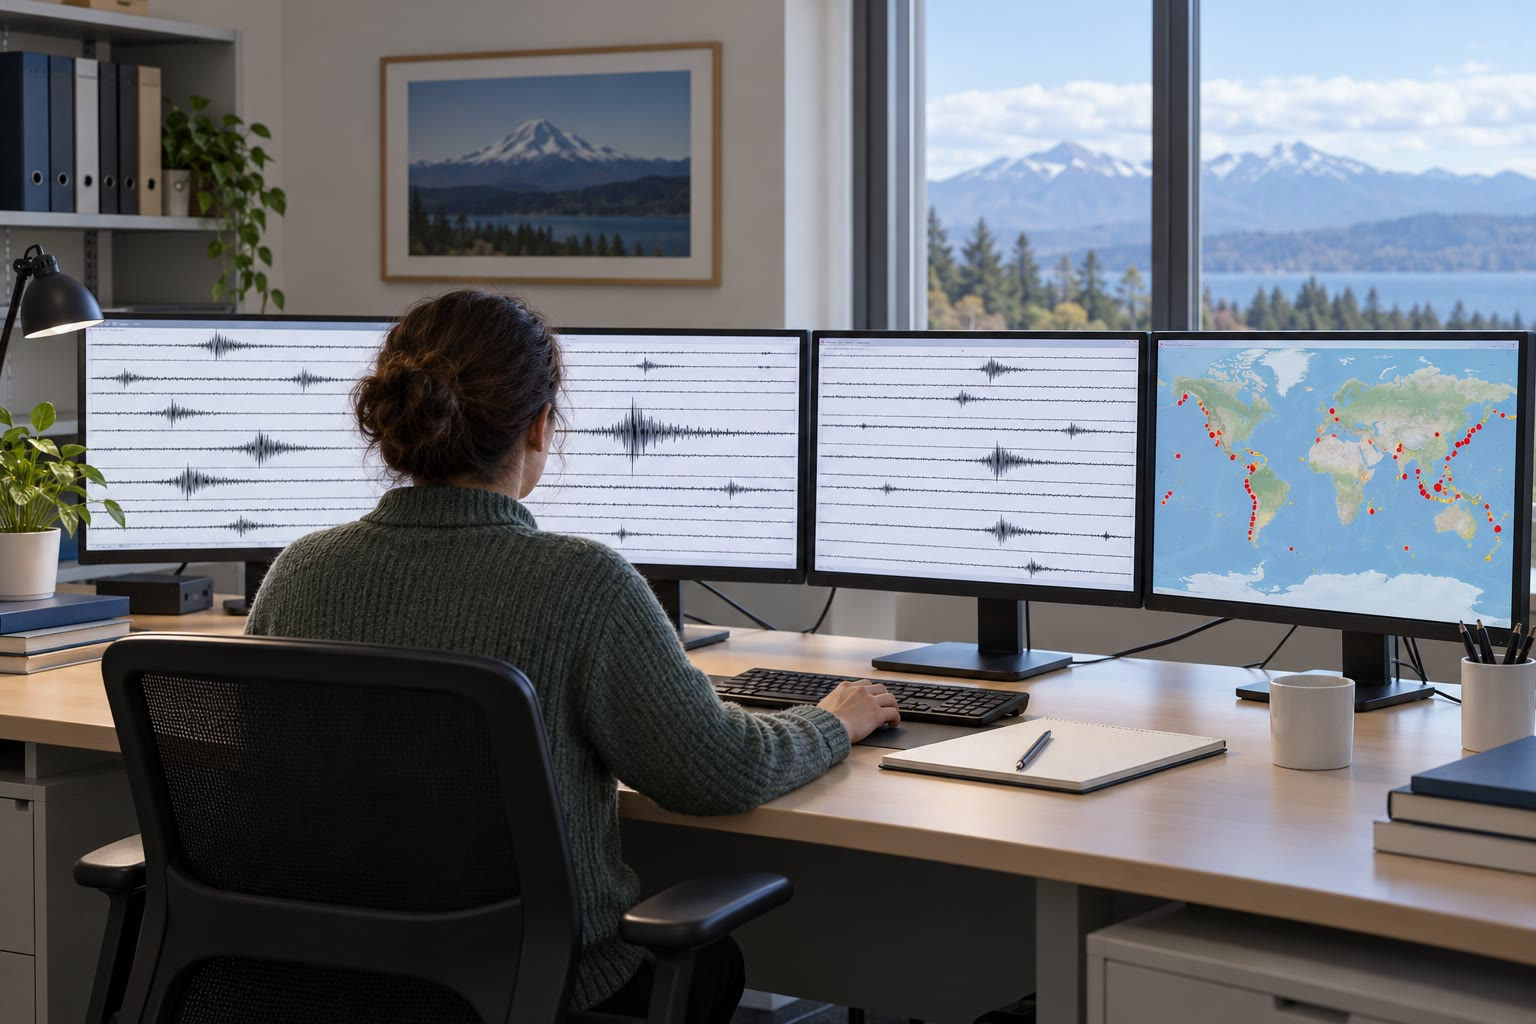
\includegraphics[width=0.66\linewidth]{images/book2/ai/g11-seismology-observatory.jpg}

{\small Num observatório de sismologia, os registros de muitas estações são
mostrados lado a lado, e os terremotos que eles localizam são marcados num
mapa-múndi (ilustração gerada por IA).}
\end{omfigure}

\section{A refração e o Moho}\label{sec:g11:seismic-structure:moho}

\subsection{A onda que corre ao longo de uma fronteira}

No interior da Terra, a velocidade das ondas sísmicas muda com a
profundidade, quase sempre gradualmente, mas em alguns lugares de uma vez.

\begin{definition}[Descontinuidade sísmica]\label{def:g11:seismic-structure:discontinuity}
Uma \emph{descontinuidade sísmica}\index{descontinuidade sismica@descontinuidade sísmica} é uma superfície
no interior da Terra através da qual a velocidade das ondas sísmicas muda
bruscamente --- numa espessura muito menor que o comprimento das ondas.
\end{definition}

Numa descontinuidade, parte de uma onda é refletida e parte é refratada.
Tome uma camada de espessura $h$ na qual as \omterm{def:g11:seismic-structure:body-waves}{ondas P} se propagam a $v_1$,
sobre uma camada na qual elas são mais rápidas, $v_2 > v_1$. Um raio que
desce com o ângulo $i$ em relação à vertical é refratado com o ângulo $r$
dado por $\sin r = (v_2/v_1)\sin
i$: ele se afasta da vertical. Quando $\sin i$ chega a $v_1/v_2$, o
raio refratado corre exatamente ao longo da fronteira. O ângulo
\[
  i_c, \qquad \sin i_c = \frac{v_1}{v_2},
\]
é o \emph{ângulo crítico}\index{angulo critico@ângulo crítico}. A onda
refratada no \omterm{ex:g11:seismic-structure:sp}{ângulo crítico} se propaga ao longo do topo da camada mais
rápida com a velocidade $v_2$ e, à medida que avança, envia ondas de volta
para cima, para a camada superior, todas com o ângulo
$i_c$: elas chegam à superfície como a \emph{onda frontal}\index{onda frontal}.

\begin{omfigure}
\begin{tikzpicture}[x=0.05cm, y=0.05cm, font=\footnotesize, >={Stealth[length=4pt]}]
% geometry from figdata/grade-11/moho_refraction.py: v1 6.2, v2 8.1, h 30 km, ic 49.9 deg
  \fill[omLithGranite!45] (-10,0) rectangle (215,-30);
  \fill[omLithPeridotite!45] (-10,-30) rectangle (215,-48);
  \draw[line width=0.6pt] (-10,0) -- (215,0);
  \draw[line width=0.9pt] (-10,-30) -- (215,-30);
  \node[anchor=west, align=left] at (218,-15) {crosta\\$v_1 = \qty{6.2}{km/s}$};
  \node[anchor=west, align=left] at (218,-39) {manto\\$v_2 = \qty{8.1}{km/s}$};
  \node[anchor=east] at (215,-26) {Moho};
  % source and station
  \fill[omDef] (0,0) circle (1.6);
  \node[anchor=south] at (0,1.5) {terremoto};
  \draw[fill=white] (197,0) -- (203,0) -- (200,5) -- cycle;
  \node[anchor=south] at (200,5) {estação};
  % direct wave
  \draw[->, omProp, line width=0.8pt] (2,-2) -- (196,-2);
  \node[anchor=south, text=omProp] at (100,0.3) {onda direta, velocidade $v_1$};
  % head wave
  \draw[omDef, line width=0.9pt] (0,0) -- (35.7,-30);
  \draw[->, omDef, line width=0.9pt] (35.7,-30) -- (100,-30);
  \draw[omDef, line width=0.9pt] (100,-30) -- (164.3,-30) -- (200,0);
  \node[anchor=north, text=omDef] at (100,-31) {ao longo do Moho a $v_2$};
  \foreach \x in {50,70,90,110,130,150} {
    \draw[->, omDef!60, densely dashed] (\x,-30) -- ++(25.5,21.5);
  }
  % critical angle
  \draw[black!60, densely dotted] (35.7,-30) -- (35.7,-8);
  \draw[black!70] (35.7,-18) arc[start angle=90, end angle=130.05, radius=12];
  \node[anchor=south east] at (33,-16) {$i_c$};
  % thickness and critical distance
  \draw[<->] (-6,0) -- (-6,-30);
  \node[anchor=east] at (-7,-15) {$h$};
\end{tikzpicture}

{\small A onda direta e a \omterm{ex:g11:seismic-structure:sp}{onda frontal} (em escala: crosta de \qty{30}{km}
de espessura). A \omterm{ex:g11:seismic-structure:sp}{onda frontal} desce com o \omterm{ex:g11:seismic-structure:sp}{ângulo crítico} $i_c$, corre ao
longo do topo do manto e volta a subir com $i_c$; ao longo de todo o seu
trajeto no \omterm{def:g11:seismic-structure:moho}{Moho}, ela envia ondas para a superfície (tracejadas). Ela não
chega a nenhuma estação mais próxima que $2h\tan i_c$, cerca de \qty{71}{km}
aqui.}
\end{omfigure}

\begin{proposition}[Tempo de percurso da onda frontal]\label{prop:g11:seismic-structure:head-wave}
Para uma fonte na superfície, uma estação à distância $x \ge 2h\tan i_c$
recebe a \omterm{ex:g11:seismic-structure:sp}{onda frontal} depois de
\[
  t(x) = \frac{x}{v_2} + \frac{2h\cos i_c}{v_1}.
\]
A sua \omterm{def:g11:seismic-structure:travel-time}{curva de tempo de percurso} é uma reta de inclinação $1/v_2$ que,
prolongada para trás, corta o eixo dos tempos no \emph{tempo de
intercepto}\index{tempo de intercepto} $t_i = 2h\cos i_c/v_1$.
\end{proposition}

\begin{proof}
O raio desce por um trecho inclinado de comprimento $h/\cos i_c$, que avança
horizontalmente $h\tan i_c$; ele faz o mesmo na subida. Entre os dois, ele
corre ao longo da fronteira por $x - 2h\tan i_c$. O tempo é
\[
  t = \frac{2h}{v_1\cos i_c} + \frac{x - 2h\tan i_c}{v_2}
    = \frac{x}{v_2} + \frac{2h}{v_1\cos i_c} - \frac{2h\sin i_c}{v_2\cos i_c}.
\]
Como $1/v_2 = \sin i_c/v_1$, os dois últimos termos dão
$\frac{2h}{v_1\cos i_c}\,(1 - \sin^2 i_c) = \frac{2h\cos i_c}{v_1}$.
\end{proof}

A onda direta chega depois de $x/v_1$: a sua curva é uma reta que passa
pela origem, mais inclinada que a reta da \omterm{ex:g11:seismic-structure:sp}{onda frontal}. Perto da fonte, a
onda direta chega primeiro; longe, a \omterm{ex:g11:seismic-structure:sp}{onda frontal}, que percorreu a maior
parte do caminho na velocidade maior, a ultrapassa.

\begin{proposition}[Distância de cruzamento]\label{prop:g11:seismic-structure:crossover}
A \omterm{ex:g11:seismic-structure:sp}{onda frontal} chega antes da onda direta além da \emph{distância de
cruzamento}\index{distancia de cruzamento@distância de cruzamento}
\[
  x_c = 2h\sqrt{\frac{v_2 + v_1}{v_2 - v_1}}.
\]
\end{proposition}

\begin{proof}
As duas chegam juntas quando $x/v_1 = x/v_2 + 2h\cos i_c/v_1$, isto é,
$x\,(v_2 - v_1)/(v_1 v_2) = 2h\cos i_c/v_1$, logo $x = 2h\cos i_c\,v_2/(v_2 -
v_1)$. Ora, $\cos i_c = \sqrt{1 - v_1^2/v_2^2} = \sqrt{(v_2 - v_1)(v_2 +
v_1)}/v_2$, portanto $x = 2h\sqrt{(v_2 + v_1)(v_2 - v_1)}/(v_2 - v_1) =
2h\sqrt{(v_2 + v_1)/(v_2 - v_1)}$. Além dela, a \omterm{ex:g11:seismic-structure:sp}{onda frontal}, cuja reta é
menos inclinada, chega primeiro.
\end{proof}

\begin{omfigure}
\begin{tikzpicture}
\begin{axis}[omrecord, width=0.78\linewidth, height=5.6cm, xmin=0, xmax=300, ymin=0, ymax=50,
  xtick={0,50,...,300}, xlabel={distância ao epicentro (\unit{km})}, ylabel={tempo de percurso (\unit{s})},
  tick label style={font=\small}, label style={font=\small}, clip=false]
% computed in figdata/grade-11/moho_refraction.py (critical_km 71.4, crossover_km 164.6, intercept_s 6.23)
\addplot[omProp, line width=0.9pt] table[x=x, y=tdirect] {figdata/out/grade-11-moho_refraction-model.dat};
\addplot[omDef, line width=0.9pt, restrict x to domain=71:300] table[x=x, y=thead] {figdata/out/grade-11-moho_refraction-model.dat};
\addplot[omDef, densely dashed, restrict x to domain=0:72] table[x=x, y=thead] {figdata/out/grade-11-moho_refraction-model.dat};
\draw[black!50, densely dotted] (axis cs:164.6,0) -- (axis cs:164.6,26.5);
\node[font=\scriptsize, anchor=north] at (axis cs:164.6,0) {$x_c$};
\fill (axis cs:0,6.23) circle (1.5pt);
\draw[black!60] (axis cs:0.8,6.6) -- (axis cs:6,12);
\node[font=\scriptsize, anchor=south west, inner sep=1pt] at (axis cs:5,12) {$t_i = \qty{6.2}{s}$};
\node[font=\small, text=omProp, anchor=south east] at (axis cs:250,41) {onda direta};
\node[font=\small, text=omDef, anchor=north west] at (axis cs:235,33) {onda frontal};
\end{axis}
\end{tikzpicture}

{\small \omterm{def:g11:seismic-structure:travel-time}{Tempos de percurso} da onda direta e da \omterm{ex:g11:seismic-structure:sp}{onda frontal} para a crosta da
figura anterior. A reta da \omterm{ex:g11:seismic-structure:sp}{onda frontal}, prolongada para trás (tracejada),
corta o eixo dos tempos no \omterm{prop:g11:seismic-structure:head-wave}{tempo de intercepto}; além da \omterm{prop:g11:seismic-structure:crossover}{distância de
cruzamento} $x_c \approx
\qty{165}{km}$, a \omterm{ex:g11:seismic-structure:sp}{onda frontal} chega primeiro.}
\end{omfigure}

\subsection{A base da crosta}

\begin{definition}[Moho]\label{def:g11:seismic-structure:moho}
A \emph{descontinuidade de Mohorovičić}\index{descontinuidade de Mohorovicic@descontinuidade de Mohorovičić}, ou
\emph{Moho}\index{Moho}, é a \omterm{def:g11:seismic-structure:discontinuity}{descontinuidade sísmica} na base da crosta, onde
a velocidade das \omterm{def:g11:seismic-structure:body-waves}{ondas P} salta de no máximo cerca de \qty{7}{km/s} para
cerca de \qty{8}{km/s}, a velocidade no topo do manto.
\end{definition}
% ledger: kayal:pn-sn, data:prem (6.8 -> 8.11 at 24.4 km)

\begin{history}[Mohorovičić e as duas ondas P, 1909]
Andrija Mohorovičić (1857--1936) descobriu, nos registros do terremoto de
1909, que além de uma certa distância --- em geral entre 100 e
\qty{150}{km} --- uma \omterm{def:g11:seismic-structure:body-waves}{onda P} fraca e mais rápida chegava antes da \omterm{def:g11:seismic-structure:body-waves}{onda P}
forte. Ele a explicou como uma onda que tinha atravessado uma rocha mais
rápida sob a crosta. Ele chamou as duas ondas de Pg (a onda direta na
crosta) e Pn (a \omterm{ex:g11:seismic-structure:sp}{onda frontal} ao longo do topo do manto), fez o mesmo para as
\omterm{def:g11:seismic-structure:body-waves}{ondas S}, e deduziu as velocidades das duas camadas e a profundidade da
fronteira entre elas. A onda Pn se propaga a cerca de \qty{8.0}{km/s}, a
velocidade do topo do manto. Os seus artigos de 1910 provaram que a crosta e
o manto são diferentes; a fronteira leva o seu nome.
\end{history}
% ledger: kayal:pn-sn, srl:mohorovicic

\begin{method}[Profundidade do Moho a partir de um diagrama de tempos de percurso]\label{met:g11:seismic-structure:moho}
\begin{enumerate}
  \item Represente os tempos das primeiras chegadas em função da distância
        ao epicentro.
  \item Trace a reta da onda direta (pela origem) e a reta da \omterm{ex:g11:seismic-structure:sp}{onda frontal};
        as suas inclinações são $1/v_1$ e $1/v_2$.
  \item Prolongue a reta da \omterm{ex:g11:seismic-structure:sp}{onda frontal} para trás até o eixo dos tempos:
        ela o corta no \omterm{prop:g11:seismic-structure:head-wave}{tempo de intercepto} $t_i$.
  \item Com $\sin i_c = v_1/v_2$, a espessura da crosta é
        $h = \dfrac{v_1\,t_i}{2\cos i_c}$.
\end{enumerate}
\end{method}

\begin{example}[Uma crosta de \qty{30}{km} de espessura]\label{ex:g11:seismic-structure:moho}
Com $v_1 = \qty{6.2}{km/s}$ e $v_2 = \qty{8.1}{km/s}$, $\sin i_c = 0.765$,
$i_c \approx \ang{49.9}$ e $\cos i_c \approx 0.644$. Um \omterm{prop:g11:seismic-structure:head-wave}{tempo de intercepto}
de \qty{6.23}{s} dá $h = 6.2 \times 6.23/(2 \times 0.644) \approx
\qty{30}{km}$. A \omterm{ex:g11:seismic-structure:sp}{onda frontal} chega à superfície pela primeira vez a
$2h\tan i_c \approx \qty{71}{km}$ e ultrapassa a onda direta além de
$x_c = 60\sqrt{14.3/1.9} \approx \qty{165}{km}$.
\end{example}
% values computed in figdata/grade-11/moho_refraction.py (ic_deg 49.9, critical_km 71.4, crossover_km 164.6)

Medido dessa maneira no mundo inteiro, o \omterm{def:g11:seismic-structure:moho}{Moho} fica apenas a cerca de
\qty{5}{km} abaixo do fundo dos oceanos. Sob os continentes, ele fica em
média a cerca de \qty{41}{km} de profundidade: cerca de \qty{30}{km} onde a
crosta foi estirada, mais de \qty{45}{km} sob as cadeias de montanhas, e até
cerca de \qty{100}{km} sob as cordilheiras mais altas. A crosta é uma pele
fina: mesmo \qty{41}{km} são menos de um por cento do raio da Terra.
% ledger: usgs:crust-thickness, cm95:crust, kayal:discontinuities

\section{O núcleo}

\subsection{Raios que se curvam}

No manto, a velocidade das ondas sísmicas aumenta com a profundidade. Um raio
que desce atravessa rochas cada vez mais rápidas e, pela lei de Snell, se
afasta um pouco mais da vertical a cada passo: o seu trajeto se curva e volta
a subir em direção à superfície. Quanto mais fundo um raio faz a curva, mais
longe do terremoto ele volta à superfície. A figura mostra raios desse tipo,
calculados com as velocidades do \omterm{def:g11:seismic-structure:reference-model}{modelo de referência da Terra}.

\begin{omfigure}
\begin{tikzpicture}
\begin{axis}[width=0.66\linewidth, height=0.66\linewidth, axis equal image, hide axis,
  xmin=-1.18, xmax=1.18, ymin=-1.18, ymax=1.2, clip=false]
% computed in figdata/grade-11/seismic_rays.py; ledger: data:prem
\fill[omLithPeridotite!25] (axis cs:0,0) circle [radius=1];
\fill[omSea!45] (axis cs:0,0) circle [radius=0.5462];
\fill[omSea!80] (axis cs:0,0) circle [radius=0.1917];
\addplot[black, line width=0.6pt, domain=0:360, samples=181] ({cos(x)}, {sin(x)});
\addplot[black!60, line width=0.4pt, domain=0:360, samples=181] ({0.5462*cos(x)}, {0.5462*sin(x)});
\addplot[black!60, line width=0.4pt, domain=0:360, samples=91] ({0.1917*cos(x)}, {0.1917*sin(x)});
\addplot[omDef, line width=0.6pt] table {figdata/out/grade-11-seismic_rays-praysmantle.dat};
\addplot[omDef!70!black, line width=0.6pt] table {figdata/out/grade-11-seismic_rays-prayscore.dat};
\addplot[omProp, line width=0.6pt] table {figdata/out/grade-11-seismic_rays-srays.dat};
% P shadow zone: 98.5 to 143.8 degrees from the source (right); S beyond 102.7 (left)
\addplot[black!80, line width=3pt, domain=-53.8:-8.5, samples=40] ({1.04*cos(x)}, {1.04*sin(x)});
\addplot[omProp!60, line width=3pt, domain=192.7:270, samples=40] ({1.04*cos(x)}, {1.04*sin(x)});
\fill[omDef] (axis cs:0,1) circle (2pt);
\node[font=\footnotesize, anchor=south] at (axis cs:0,1.04) {terremoto};
\node[font=\footnotesize, anchor=west, align=left] at (axis cs:1.07,-0.42) {sem P direta\\(\ang{99}--\ang{144})};
\node[font=\footnotesize, anchor=east, align=right] at (axis cs:-1.07,-0.62) {sem S direta\\além de \ang{103}};
\node[font=\footnotesize, text=omDef, anchor=south west] at (axis cs:0.55,0.8) {P};
\node[font=\footnotesize, text=omProp, anchor=south east] at (axis cs:-0.55,0.8) {S};
\node[font=\scriptsize] at (axis cs:-0.5,-0.62) {manto};
\node[font=\scriptsize] at (axis cs:-0.3,0.2) {núcleo externo};
\draw[black!70] (axis cs:-0.1,-0.06) -- (axis cs:-0.26,-0.22);
\node[font=\scriptsize, anchor=north east, inner sep=1pt] at (axis cs:-0.24,-0.22) {núcleo interno};
\end{axis}
\end{tikzpicture}

{\small Raios de um terremoto no topo da Terra, calculados com as
velocidades do modelo de referência. À direita: raios P que fazem a curva no
manto, até cerca de \ang{99}, e raios P que atravessam o núcleo e saem além
de cerca de \ang{144}; entre os dois, nenhum raio P chega diretamente. À
esquerda: raios S, que fazem a curva no manto; nenhum atravessa o núcleo
externo líquido, e nenhuma \omterm{def:g11:seismic-structure:body-waves}{onda S} direta chega além de cerca de \ang{103}.}
\end{omfigure}

\subsection{A zona de sombra e o núcleo externo líquido}

Em 1906, o sismólogo Oldham percebeu que as \omterm{def:g11:seismic-structure:body-waves}{ondas P} registradas do outro lado
da Terra em relação a um terremoto chegavam atrasadas em comparação com os
tempos esperados, e propôs um núcleo central no qual elas se propagam mais
devagar. Em 1912, Gutenberg mostrou que as \omterm{def:g11:seismic-structure:body-waves}{ondas P} não chegam a toda uma
faixa de distâncias, entre cerca de \ang{105} e \ang{143}, com chegadas
fortes logo além de \ang{143}; em 1914, ele situou o topo do núcleo a
\qty{2900}{km} de profundidade.
% ledger: kayal:discontinuities, kayal:shadow

\begin{definition}[Zona de sombra]\label{def:g11:seismic-structure:shadow-zone}
A \emph{zona de sombra}\index{zona de sombra} de uma onda sísmica é a faixa
de distâncias epicentrais que a onda não consegue alcançar diretamente a
partir de um terremoto, porque o núcleo a desvia ou a detém.
\end{definition}

Os raios a explicam. Os raios P que fazem a curva logo acima do núcleo
voltam à superfície a cerca de \ang{100} do terremoto. Um raio que desce um
pouco mais inclinado entra no núcleo, onde a velocidade P cai bruscamente de
\qty{13.7}{km/s} para cerca de \qty{8.1}{km/s}: pela lei de Snell, ele se
inclina \emph{em direção} à vertical, atravessa o núcleo e sai muito mais
longe, além de cerca de \ang{144}. Nenhum raio P que faz a curva no manto e
nenhum raio P que atravessa o núcleo cai entre os dois. No modelo de
referência, a \omterm{def:g11:seismic-structure:shadow-zone}{zona de sombra} P vai de \ang{98.5} a \ang{143.8}, perto dos
\ang{105}--\ang{143} de Gutenberg.
% ledger: kayal:shadow, data:prem (vp_above_cmb 13.72, vp_below_cmb 8.06); computed in
% figdata/grade-11/seismic_rays.py (shadow_start_deg 98.5, shadow_end_pkp_deg 143.8)

As \omterm{def:g11:seismic-structure:body-waves}{ondas S} dizem mais. Nenhuma \omterm{def:g11:seismic-structure:body-waves}{onda S} atravessa o núcleo externo: o núcleo
externo não transmite ondas de cisalhamento, logo ele é líquido. Em
consequência, nenhuma \omterm{def:g11:seismic-structure:body-waves}{onda S} chega diretamente além de cerca de \ang{103} no
modelo de referência --- em todo o lado oposto da Terra.
% ledger: kayal:outer-core-liquid; computed in figdata/grade-11/seismic_rays.py (s_direct_max_deg 102.7)

\begin{definition}[Limite manto--núcleo; limite do núcleo interno]\label{def:g11:seismic-structure:core}
O \emph{limite manto--núcleo}\index{limite manto--nucleo@limite manto--núcleo} é a \omterm{def:g11:seismic-structure:discontinuity}{descontinuidade
sísmica} entre o manto sólido e o núcleo externo líquido, a uma profundidade
de \qty{2891}{km}; ali, a velocidade P cai de cerca de \qty{13.7}{km/s} para
cerca de \qty{8.1}{km/s}, e as \omterm{def:g11:seismic-structure:body-waves}{ondas S} param. O \emph{limite do núcleo
interno}\index{limite do nucleo interno@limite do núcleo interno}, a uma profundidade de \qty{5150}{km}, separa
o núcleo externo líquido do núcleo interno sólido; ali, a velocidade P salta
de cerca de \qty{10.4}{km/s} para cerca de \qty{11.0}{km/s}.
\end{definition}
% ledger: data:prem, prem:cmb, prem:icb (Book 3 rows); values in figdata/grade-11/prem_profiles.py

A \omterm{def:g11:seismic-structure:shadow-zone}{zona de sombra} não é completamente silenciosa: \omterm{def:g11:seismic-structure:body-waves}{ondas P} fracas chegam a
ela. Inge Lehmann as explicou em 1936 com um núcleo interno sólido, no qual
as \omterm{def:g11:seismic-structure:body-waves}{ondas P} se propagam mais depressa (Livro 1, 6º ano). Os raios mostram
como. Um raio P que chega ao núcleo interno se afasta da vertical onde a
velocidade salta para cima, como no \omterm{def:g11:seismic-structure:moho}{Moho}, e sai do núcleo mais cedo: no
modelo de referência, os raios que atravessam o núcleo interno chegam à
superfície a partir de cerca de \ang{121}, dentro da \omterm{def:g11:seismic-structure:shadow-zone}{zona de sombra} (curva
pontilhada da figura dos \omterm{def:g11:seismic-structure:travel-time}{tempos de percurso}).
% ledger: nbi:lehmann-1936 (Book 1 row), kayal:lehmann; computed in
% figdata/grade-11/seismic_rays.py (pkikp_min_deg 121.4)

\section{Um modelo de referência da Terra}\label{sec:g11:seismic-structure:model}

Reunidos, milhões de \omterm{def:g11:seismic-structure:travel-time}{tempos de percurso} dão a velocidade das \omterm{def:g11:seismic-structure:body-waves}{ondas P} e S em
cada profundidade. As suas velocidades dependem da rocha e da sua
densidade, e a massa total da Terra fixa a sua densidade média; juntas, elas
dão também a densidade em cada profundidade.
% ledger: data:prem, prem:constraints (Book 3 row)

\begin{definition}[Modelo de referência da Terra]\label{def:g11:seismic-structure:reference-model}
Um \emph{modelo de referência da Terra}\index{modelo de referencia da Terra@modelo de referência da Terra} é uma tabela da
velocidade das \omterm{def:g11:seismic-structure:body-waves}{ondas P}, da velocidade das \omterm{def:g11:seismic-structure:body-waves}{ondas S} e da densidade em função
da profundidade, a mesma em todas as direções, escolhida para concordar com
os \omterm{def:g11:seismic-structure:travel-time}{tempos de percurso} observados das ondas sísmicas e com a massa da Terra.
\end{definition}

O mais usado é o Preliminary Reference Earth Model (PREM), publicado por
A.~M.~Dziewonski e D.~L.~Anderson em 1981. Os raios e os \omterm{def:g11:seismic-structure:travel-time}{tempos de percurso}
deste capítulo foram calculados com ele: o \omterm{def:g11:seismic-structure:travel-time}{tempo de percurso} P a \ang{60},
por exemplo, sai \qty{607}{s}, contra \qty{608}{s} observados.
% ledger: data:prem, auspass:surftim; computed in figdata/grade-11/seismic_rays.py (p_60_s 607.2)

\begin{omfigure}
\begin{tikzpicture}
\begin{axis}[omrecord, width=0.86\linewidth, height=6.2cm, xmin=0, xmax=6371, ymin=0, ymax=14.5,
  xtick={0,1000,...,6000}, ytick={0,2,...,14}, scaled x ticks=false,
  xticklabel style={/pgf/number format/1000 sep={\,}},
  xlabel={profundidade (\unit{km})}, ylabel={velocidade (\unit{km/s}) ou densidade (\unit{g/cm^3})},
  tick label style={font=\small}, label style={font=\small}, clip=false]
% computed in figdata/grade-11/prem_profiles.py; ledger: data:prem
\addplot[omDef, line width=0.9pt] table[x=depth, y=vp] {figdata/out/grade-11-prem_profiles-profile.dat};
\addplot[omProp, line width=0.9pt] table[x=depth, y=vs] {figdata/out/grade-11-prem_profiles-profile.dat};
\addplot[black, line width=0.9pt, densely dashed] table[x=depth, y=rho] {figdata/out/grade-11-prem_profiles-profile.dat};
\foreach \d in {670,2891,5149.5} {\edef\temp{\noexpand\draw[black!40, densely dotted] (axis cs:\d,0) -- (axis cs:\d,14.5);}\temp}
\node[font=\scriptsize, anchor=south, align=center] at (axis cs:2891,14.5) {limite\\manto--núcleo};
\node[font=\scriptsize, anchor=south, align=center] at (axis cs:5149.5,14.5) {limite do\\núcleo interno};
\node[font=\scriptsize, anchor=south] at (axis cs:670,14.5) {\qty{670}{km}};
\node[font=\small, text=omDef, anchor=south] at (axis cs:1800,12.4) {ondas P};
\node[font=\small, text=omProp, anchor=south] at (axis cs:1800,7.0) {ondas S};
\node[font=\small, anchor=north] at (axis cs:1800,4.5) {densidade};
\node[font=\scriptsize, align=center] at (axis cs:4000,1.9) {sem ondas S:\\líquido};
\end{axis}
\end{tikzpicture}

{\small As velocidades das \omterm{def:g11:seismic-structure:body-waves}{ondas P} e S e a densidade em função da
profundidade no Preliminary Reference Earth Model (Dziewonski e Anderson,
1981). As linhas pontilhadas marcam as principais descontinuidades abaixo do
\omterm{def:g11:seismic-structure:moho}{Moho}, que é raso demais para aparecer nesta escala.}
\end{omfigure}

Lendo o modelo de cima para baixo:
\begin{itemize}
  \item a crosta, com velocidades P de 5.8 a \qty{6.8}{km/s}, termina no
        \omterm{def:g11:seismic-structure:moho}{Moho} (\qty{24.4}{km} neste modelo médio);
  \item no manto, as velocidades sobem com a profundidade, com saltos
        bruscos menores, os maiores perto de \qty{400}{km} e de
        \qty{670}{km};
  \item a \qty{2891}{km}, a velocidade S cai a zero e a velocidade P cai
        mais de \qty{5}{km/s}: o núcleo externo líquido;
  \item a \qty{5150}{km}, as \omterm{def:g11:seismic-structure:body-waves}{ondas S} voltam a existir: o núcleo interno
        sólido, de \qty{1220}{km} de raio.
\end{itemize}
% ledger: data:prem (discontinuities in figdata/grade-11/prem_profiles.py)

A densidade sobe de \qty{2.6}{g/cm^3} na crosta para \qty{5.6}{g/cm^3} na
base do manto, depois salta para \qty{9.9}{g/cm^3} no topo do núcleo e chega
a \qty{13.1}{g/cm^3} no centro. A densidade média de todo o modelo é de
\qty{5.5}{g/cm^3}, o dobro da das rochas da crosta: o interior profundo, e
sobretudo o núcleo, é feito de um material muito mais denso que a
superfície. O núcleo contém cerca de um terço da massa da Terra.
% ledger: data:prem, prem:cmb, prem:centre (Book 3 rows); computed in
% figdata/grade-11/prem_profiles.py (mean_density 5.52; core mass fraction 0.32)

\section{Exercícios}

\begin{exercise}[$\star$]\label{exo:g11:seismic-structure:1}
Dê duas diferenças entre as \omterm{def:g11:seismic-structure:body-waves}{ondas P} e as \omterm{def:g11:seismic-structure:body-waves}{ondas S}. Qual delas é registrada
primeiro por um sismômetro, e por quê?
\end{exercise}

\begin{exercise}[$\star$]\label{exo:g11:seismic-structure:2}
Uma estação fica a \ang{40} de um epicentro. A que distância ela está,
medida ao longo da superfície? A quantos graus fica uma estação a
\qty{8900}{km} de um epicentro?
\end{exercise}

\begin{exercise}[$\star$]\label{exo:g11:seismic-structure:3}
Os \omterm{def:g11:seismic-structure:travel-time}{tempos de percurso} observados a \ang{40} são de \qty{456}{s} para P e
\qty{822}{s} para S. Converta-os em minutos e segundos, e dê o atraso S--P.
\end{exercise}

\begin{exercise}[$\star$]\label{exo:g11:seismic-structure:4}
Uma crosta na qual as \omterm{def:g11:seismic-structure:body-waves}{ondas P} se propagam a \qty{6.0}{km/s} repousa sobre um
manto onde elas se propagam a \qty{8.0}{km/s}. Calcule o \omterm{ex:g11:seismic-structure:sp}{ângulo crítico}.
\end{exercise}

\begin{exercise}[$\star$]\label{exo:g11:seismic-structure:5}
No modelo de referência, o \omterm{def:g11:seismic-structure:core}{limite manto--núcleo} fica a \qty{2891}{km} de
profundidade e o \omterm{def:g11:seismic-structure:core}{limite do núcleo interno} a \qty{5150}{km}; o raio da Terra
é de \qty{6371}{km}. Calcule a espessura do núcleo externo, o raio do núcleo
e o raio do núcleo como fração do raio da Terra.
\end{exercise}

\begin{exercise}[$\star\star$]\label{exo:g11:seismic-structure:6}
Os atrasos S--P observados são de \qty{224}{s} a \ang{20}, \qty{298}{s} a
\ang{30}, \qty{366}{s} a \ang{40}, \qty{431}{s} a \ang{50} e
\qty{493}{s} a \ang{60}. Uma estação registra uma \omterm{def:g11:seismic-structure:body-waves}{onda S} 6~minutos e
6~segundos depois da \omterm{def:g11:seismic-structure:body-waves}{onda P}. A que distância está o terremoto, em graus e
em quilômetros? Por que uma única estação não consegue dizer onde está o
terremoto?
\end{exercise}

\begin{exercise}[$\star\star$]\label{exo:g11:seismic-structure:7}
Com as velocidades do \cref{exo:g11:seismic-structure:4} e uma crosta de
\qty{35}{km} de espessura, calcule os \omterm{def:g11:seismic-structure:travel-time}{tempos de percurso} da onda direta e
da \omterm{ex:g11:seismic-structure:sp}{onda frontal} numa estação a \qty{200}{km} do epicentro. Qual chega
primeiro?
\end{exercise}

\begin{exercise}[$\star\star$]\label{exo:g11:seismic-structure:8}
Para a crosta do \cref{exo:g11:seismic-structure:7}, calcule a distância
crítica $2h\tan i_c$ e a \omterm{prop:g11:seismic-structure:crossover}{distância de cruzamento}. Verifique que a resposta ao
\cref{exo:g11:seismic-structure:7} concorda.
\end{exercise}

\begin{exercise}[$\star\star$]\label{exo:g11:seismic-structure:9}
Sob um oceano, uma crosta de \qty{6}{km} de espessura, na qual as \omterm{def:g11:seismic-structure:body-waves}{ondas P} se
propagam a \qty{6.5}{km/s}, repousa sobre um manto a \qty{8.0}{km/s}.
Calcule o \omterm{ex:g11:seismic-structure:sp}{ângulo crítico}, o \omterm{prop:g11:seismic-structure:head-wave}{tempo de intercepto} e a \omterm{prop:g11:seismic-structure:crossover}{distância de cruzamento}.
Por que as estações precisam estar muito mais próximas umas das outras para
encontrar o \omterm{def:g11:seismic-structure:moho}{Moho} sob um oceano do que sob um continente?
\end{exercise}

\begin{exercise}[$\star\star$]\label{exo:g11:seismic-structure:10}
Um raio P no manto mais profundo, onde se propaga a \qty{13.7}{km/s},
encontra o \omterm{def:g11:seismic-structure:core}{limite manto--núcleo} a \ang{30} da perpendicular. Abaixo do
limite, a velocidade P é de \qty{8.06}{km/s}. Calcule o ângulo do raio
refratado. O raio se inclina em direção à perpendicular ou se afasta dela?
Use isso para explicar por que os raios P que entram no núcleo saem longe do
terremoto.
\end{exercise}

\begin{exercise}[$\star\star$]\label{exo:g11:seismic-structure:11}
No modelo de referência, uma \omterm{def:g11:seismic-structure:body-waves}{onda P} que desce em linha reta passando pelo
centro leva \qty{1210}{s} para chegar ao ponto oposto da Terra. Quanto tempo
ela levaria se percorresse todo o diâmetro (\qty{12742}{km}) a
\qty{13.7}{km/s}, a velocidade P na base do manto? O que Oldham concluiu
desses atrasos?
\end{exercise}

\begin{exercise}[$\star\star\star$]\label{exo:g11:seismic-structure:12}
(1) A partir da \cref{prop:g11:seismic-structure:head-wave}, mostre que a
espessura da crosta é
\[
  h = \frac{t_i\,v_1 v_2}{2\sqrt{v_2^2 - v_1^2}}.
\]
(2) Aplique-a a $t_i = \qty{6.23}{s}$, $v_1 = \qty{6.2}{km/s}$ e
$v_2 = \qty{8.1}{km/s}$.
\end{exercise}

\begin{exercise}[$\star\star\star$]\label{exo:g11:seismic-structure:13}
A densidade média da Terra é de \qty{5.52}{g/cm^3}. Trate a Terra como um
núcleo de raio \qty{3480}{km} e densidade uniforme $\rho_c$, dentro de um
manto e de uma crosta de densidade uniforme \qty{4.45}{g/cm^3} (a média do
modelo de referência). (1) Que fração do volume da Terra é o núcleo? (2)
Calcule $\rho_c$. (3) Compare com a densidade no topo do núcleo no modelo de
referência, \qty{9.9}{g/cm^3}, e com a densidade da crosta.
\end{exercise}

\begin{exercise}[$\star\star\star$]\label{exo:g11:seismic-structure:14}
A \omterm{def:g11:seismic-structure:shadow-zone}{zona de sombra} P de Gutenberg vai de \ang{105} a \ang{143}. (1) Dê os seus
limites em quilômetros ao longo da superfície. (2) Numa esfera, a área entre
as distâncias angulares $a$ e $b$ de um ponto é a fração $(\cos a - \cos
b)/2$ de toda a superfície. Que fração da superfície da Terra não recebe
nenhuma \omterm{def:g11:seismic-structure:body-waves}{onda P} direta de um dado terremoto? (3) Por que cada terremoto tem a
sua própria \omterm{def:g11:seismic-structure:shadow-zone}{zona de sombra}?
\end{exercise}

\begin{exercise}[$\star\star\star$]\label{exo:g11:seismic-structure:15}
Sob uma alta cadeia de montanhas, um levantamento de refração encontra $v_1 =
\qty{6.3}{km/s}$, $v_2 = \qty{8.1}{km/s}$ e um \omterm{prop:g11:seismic-structure:head-wave}{tempo de intercepto} de
\qty{9.5}{s}. (1) Calcule a espessura da crosta ali. (2) Que \omterm{prop:g11:seismic-structure:head-wave}{tempo de
intercepto} daria uma crosta de \qty{30}{km} de espessura com as mesmas
velocidades? (3) Compare com a espessura média da crosta continental.
\end{exercise}

\section{Problema: encontrar o Moho}

\begin{problem}[{Problema de fim de semana --- a profundidade da crosta a partir de quinze estações}]
\label{pb:g11:seismic-structure:1}
% readings computed in figdata/grade-11/moho_refraction.py (part stations; invented region,
% v1 6.2, v2 8.1, h 30 km, reading errors of up to 0.1 s); ledger: kayal:pn-sn, usgs:crust-thickness
Um pequeno terremoto ocorre a uma profundidade muito rasa sob um continente.
Quinze estações dispostas numa linha reta a partir do epicentro registram os
instantes de chegada da primeira \omterm{def:g11:seismic-structure:body-waves}{onda P} e, onde é possível lê-los, de uma
segunda. As leituras abaixo são inventadas, mas calculadas como um
levantamento real as encontraria, ao décimo de segundo. Pg é a onda que se
propaga pela crosta, Pn a que correu ao longo do topo do manto.

\begin{center}
\small
\begin{tabular}{|c|c|c||c|c|c|}
\hline
distância (\unit{km}) & Pg (\unit{s}) & Pn (\unit{s}) & distância (\unit{km}) & Pg (\unit{s}) & Pn (\unit{s}) \\ \hline
20 & 3.3 & --- & 180 & 29.0 & 28.5 \\ \hline
40 & 6.5 & --- & 200 & 32.3 & 30.9 \\ \hline
60 & 9.7 & --- & 220 & --- & 33.3 \\ \hline
80 & 12.8 & 16.2 & 240 & --- & 35.8 \\ \hline
100 & 16.1 & 18.6 & 260 & --- & 38.3 \\ \hline
120 & 19.3 & 21.1 & 280 & --- & 40.8 \\ \hline
140 & 22.6 & 23.6 & 300 & --- & 43.2 \\ \hline
160 & 25.8 & 26.0 & & & \\ \hline
\end{tabular}
\end{center}

\medskip
\noindent\textbf{Parte I --- A onda direta.}
\begin{enumerate}
  \item Em papel milimetrado, represente os tempos Pg e Pn em função da
        distância (\qty{1}{cm} para \qty{20}{km} e para \qty{5}{s}). Como se
        dispõem os pontos Pg?
  \item Por que a reta Pg passa perto da origem?
  \item Usando as estações a 20 e a \qty{200}{km}, calcule a inclinação da
        reta Pg em segundos por quilômetro.
  \item Deduza a velocidade $v_1$ das \omterm{def:g11:seismic-structure:body-waves}{ondas P} na crosta.
  \item Se a crosta continuasse, quando a onda Pg chegaria à estação a
        \qty{300}{km}?
\end{enumerate}

\medskip
\noindent\textbf{Parte II --- A onda refratada.}
\begin{enumerate}[resume]
  \item Usando as estações a 100 e a \qty{300}{km}, calcule a inclinação da
        reta Pn e a velocidade $v_2$ das \omterm{def:g11:seismic-structure:body-waves}{ondas P} sob a crosta.
  \item Compare $v_2$ com a velocidade da onda Pn que Mohorovičić mediu,
        cerca de \qty{8.0}{km/s}. Que rocha fica sob a crosta?
  \item Calcule o \omterm{ex:g11:seismic-structure:sp}{ângulo crítico} $i_c$.
  \item Nenhuma estação mais próxima que \qty{80}{km} registra uma onda Pn.
        Usando a \cref{prop:g11:seismic-structure:head-wave}, explique por
        que existe uma distância mínima a partir da qual a \omterm{ex:g11:seismic-structure:sp}{onda frontal} pode
        ser registrada.
  \item Entre 80 e \qty{160}{km}, Pn chega depois de Pg. Por que ela ainda é
        registrada?
\end{enumerate}

\medskip
\noindent\textbf{Parte III --- O cruzamento.}
\begin{enumerate}[resume]
  \item Pela tabela, entre quais duas estações a primeira onda a chegar
        passa de Pg para Pn?
  \item Escreva as equações das duas retas, usando os pontos a \qty{20}{km}
        (Pg) e a \qty{100}{km} (Pn).
  \item Calcule a distância em que as duas retas se cruzam.
  \item Além de \qty{200}{km}, nenhuma estação registra Pg como uma onda
        separada. Que onda uma estação a \qty{250}{km} registra primeiro, e
        quando?
\end{enumerate}

\medskip
\noindent\textbf{Parte IV --- A profundidade do Moho.}
\begin{enumerate}[resume]
  \item Prolongue a reta Pn para trás até o eixo dos tempos: qual é o \omterm{prop:g11:seismic-structure:head-wave}{tempo
        de intercepto} $t_i$?
  \item Calcule $\cos i_c$, e a espessura $h$ da crosta pelo
        \cref{met:g11:seismic-structure:moho}.
  \item Verifique: com esse $h$, calcule a \omterm{prop:g11:seismic-structure:crossover}{distância de cruzamento} com a
        \cref{prop:g11:seismic-structure:crossover} e compare com a
        questão~13.
  \item Verifique de novo: calcule a distância crítica $2h\tan i_c$ e compare
        com a estação mais próxima que registra Pn.
  \item Os sismólogos dão $h$ apenas a alguns quilômetros. Por que um valor
        mais fino não se justifica?
  \item Conclua: a que profundidade fica o \omterm{def:g11:seismic-structure:moho}{Moho} sob esta região? A crosta
        aqui é fina ou espessa para um continente?
\end{enumerate}
\end{problem}
